\section{Introduction}
The SPV clients described in the Bitcoin paper need to process only the block headers of the chain in order to synchronize. This is much more efficient compared to the synchronization of a full node, however it still requires processing data which grow linearly with the size of the chain.

Superblock NIPoPoWs provide synchronization and up-to-date chain information with only polylogarithmic data to the size of the chain. Let us describe the underlying primitive and try to provide some intuition about it.

As already explained, each block appended to the chain must contain an appropriate nonce value, so that the hash of the whole block is a number lower than a specific threshold. Assuming $\text{difficulty} = 1/T$ then for a block's hash $\text{id}$ it must hold that $\dfrac{\text{id}}{T} < 1$. This is illustrated in the part I of Figure~\ref{fig:pow}. Remember that $\kappa$ is the length of the hash function output.

\begin{figure}[h!]
	\begin{center}
		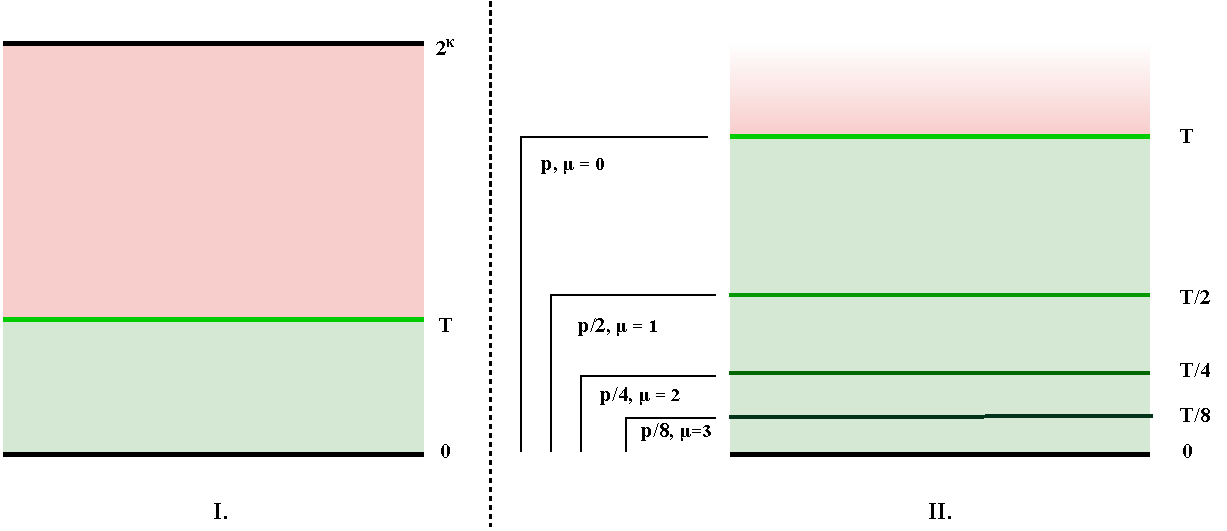
\includegraphics[width=\columnwidth]{figures/pow.pdf}
	\end{center}
	\caption{Graphical representation of PoW domain. I. valid blocks ids lie in the green section. II. blocks of higher level are generated with lower probability.}
	\label{fig:pow}
\end{figure}

Note that because of the Random Oracle model for the hash function, the outputs of the PoW attempts are uniformly distributed in the domain $\{0, 2^{\kappa} \}$.
The values regarding any subdomain follow uniform distribution too.
In essence, a block $b$ with $id < T$ is generated with probability $p = \dfrac{T}{2^\kappa}$, while a block $b_1$ with $id_1 < \dfrac{T}{2}$ is generated with probability $p_1 = \dfrac{T}{2 \cdot 2^\kappa} $ or $p_1 = \dfrac{p}{2}$. As you can see it seems that $b_1$ is a ``luckier'' block than block $b$, and we could even say that it is twice as lucky since such a block is generated half of the times that $b$ is, in expectation. This can be generalized to the following form: a block $b'$ with $\text{id}' < \dfrac{T}{2^\mu}$ is generated with probability $p' = \dfrac{p}{2^\mu}$. We call $\mu$ the level of the block $b'$.
It should now be obvious that blocks of high levels appear rarely in the chain according to their level. The higher the level $\mu$, the more rare the blocks of that level in the chain. Part II of Figure~\ref{fig:pow} illustrates this result.

From all the above we can conclude to the following. All blocks in the chain are level 0. Blocks of level $\mu$ are called $\mu\text{-superblocks}$, while it holds that $\mu$-superblocks for $\mu > 0$ are also $(\mu -1)$-superblocks. The level of a block is given as $\mu = \lfloor log(T) - log(id(B)) \rfloor$ and denoted $level(B)$. By convention, for the genesis block we set $id = 0$ and $\mu = \infty$.

The important observation on the superblocks is that they are expected to appear in the chain with a constant frequency according to their level. This is validated for the bitcoin blockchain in~\cite{compactsuperblocks}. In a blockchain protocol execution it is expected that half of the blocks will be of level 1, 1/4 of the blocks will be of level 2, 1/8 of the blocks of level 3 and, generally, $1 / 2^\mu$ blocks will be of level $\mu$. In expectation the number of superblock levels appearing in a chain $\chain$ will be $\Theta(log(\chain))$. Figure~\ref{fig:superblock_distribution} illustrates the blockchain superblocks starting from level 1 and going up to level 4 in the case that superblocks are distributed exactly according to expectation. Each level contains half of the blocks of the level below~\cite{nipopows}.

\begin{figure}[h!]
	\begin{center}
		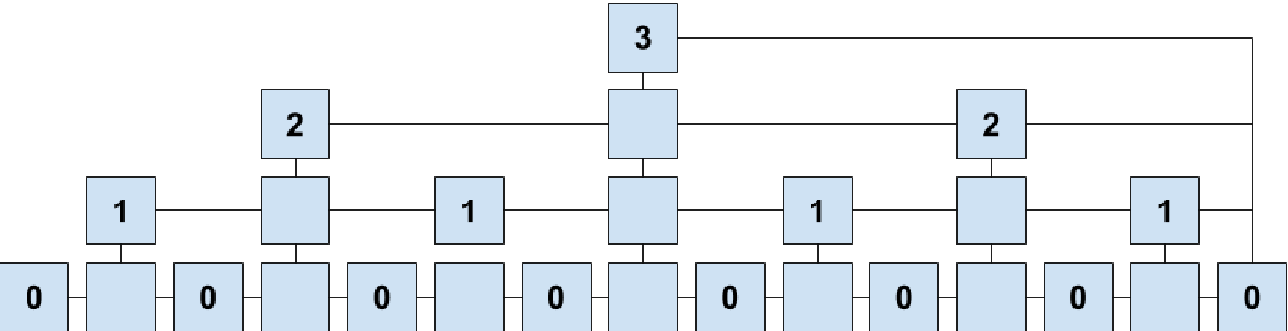
\includegraphics[width=0.8\columnwidth]{figures/superblock-distribution.pdf}
	\end{center}
	\caption{Ideal superblock distribution. Higher levels have achieved higher difficulty during mining~\cite{nipopows}.}
	\label{fig:superblock_distribution}
\end{figure}

The main idea behind superblock lightclients should now seem straightforward. Since one $\mu-$superblock roughly represents $2^\mu$ 0-level blocks, why don't we provide only these very lucky blocks instead of communicating the headers of all blocks in the chain in order to synchronize?